-----------------------------
\section{A Physically-based Manufactured Solution for FANS--SA Equations}\label{oliver}
%The goal of this work is to develop a manufactured solution for the FANS-SA equations. 
 To exercise all of the terms in the equation, the solution must satisfy the no slip wall boundary condition for at least
some portion of the boundary.  To avoid pathological behavior in the solution and required source terms, we strive to make the manufactured
solution reasonably resemble the inner portion (viscous sublayer + logarithmic layer) of a zero pressure gradient boundary layer.  To
accomplish this goal, the manufactured solution is built using well-known correlations for turbulent boundary layers.  The
manufactured solution is developed in Sections~\ref{sec:velocity_field} through~\ref{sec:sa_state_field}.
Some of the derivatives required to compute the manufactured source
terms are given in Section~\ref{sec:derivatives}.  The
behavior of the solution is shown graphically for particular values of
the constant parameters in Section~\ref{sec:soln_plots}.  To check the
behavior of the SA model terms, the SA model budget is computed and
shown in Section~\ref{sec:sa_budget}.


%-------------------------------------------------
\subsection{Velocity Field} \label{sec:velocity_field}

\subsubsection{Streamwise Velocity}
For the streamwise velocity, we construct the solution by working
backward from the van Driest transformation.  Inverting the adiabatic
wall form of the van Driest transformation~\cite{VanDriest_1956, White1991} gives
%
\begin{equation} \label{eqn:streamwise_velocity}
u = \frac{u_{\infty}}{A} \sin \left( \frac{A}{u_{\infty}} u_{eq} \right),
\end{equation}
% 
where $u_{\infty}$, $A = \sqrt{1 - T_{\infty}/T_{aw}}$,
$T_{\infty}$, and $T_{aw}$ are constants, and $u_{eq}$ is the van
Driest equivalent velocity.  The van Driest equivalent velocity can be
computed from the friction velocity $u_{\tau}$ and the
non-dimensionalized van Driest velocity $u_{eq}^+ \equiv
u_{eq}/u_{\tau}$.  Clearly,
%
\begin{equation}\label{eqn:van_Driest}
u_{eq} = u_{\tau} u_{eq}^+.
\end{equation}
% 
Thus, to specify the velocity, one must specify $u_{\tau}$ and
$u_{eq}^+$.  The friction velocity can be determined from the skin
friction coefficient:
%
\begin{equation} \label{eqn:utau}
u_{\tau} \equiv \sqrt{\frac{\tau_{w}}{\rho_w}} = u_{\infty} \sqrt{\frac{c_f}{2}}.
\end{equation}
% 
We model the skin friction coefficient using the compressibility
transformation idea of Spalding and Chi~\cite{Chi_Spalding_1966} and a correlation for
the incompressible skin friction.  Specifically,
%
\begin{equation} \label{eqn:skin_friction}
c_f = \frac{1}{F_c} c_{f,inc}\left( \frac{1}{F_c} Re_x \right),
\end{equation}
%
where
%
\begin{equation} \label{eqn:Fc}
F_c = \frac{T_{aw}/T_{\infty} - 1}{ \left( \sin^{-1} A \right)^2}
\end{equation}
%
is a constant and $c_{f,inc}$ is a correlation for the incompressible
skin friction.  Specifically, we choose a power law for the
incompressible skin friction coefficient:
%
\begin{equation} \label{eqn:cf_inc}
c_{f,inc}(Re_x) = C_{cf} Re_{x}^{-1/7},
\end{equation}
%
where $C_{cf}$ is a constant.

Finally, to complete the manufactured solution, we set $u^+_{eq}$
using the velocity profile model of Cebeci and Bradshaw \cite{Cebeci_Bradshaw_1980}:
%
\begin{equation} \label{eqn:nd_incomp_profile}
u_{eq}^+ = \frac{1}{\kappa} \log \left( 1 + \kappa y^+ \right) + C_1 \left[ 1 - e^{-y^+/\eta_1} - \frac{y^+}{\eta_1} e^{-y^+ b} \right],
\end{equation}
%
where $\kappa$,  $\eta_1$ and $b$ are constants, and
%
\begin{equation} \label{eqn:C1}
C_1 = -(1/\kappa) \log(\kappa) + C.
\end{equation}

%
\begin{equation}
y^+ \equiv \frac{y}{\ell_v},
\end{equation}
%
and
%
\begin{equation} \label{eqn:visc_length}
\ell_v \equiv \frac{\nu_w}{u_{\tau}}.
\end{equation}
%


\subsubsection{Wall-normal Velocity}
Based on a crude order of magnitude analysis of the continuity
equation, the wall-normal velocity component is set to:

%
\begin{equation} \label{eqn:wall_normal_vel}
v = -\eta_v \dd{u_{\tau}}{x} y ,
\end{equation}
%
where $\eta_v$ is a user-specified parameter.

%-------------------------------------------------
\subsection{Thermodynamic State} \label{sec:thermodynamic_state}
For the mean temperature, we write:
%
\begin{equation} \label{eqn:temp_vel}
T = T_{\infty} \left[ 1 + r_T \frac{\gamma - 1}{2} M_{\infty}^2 \left( 1 - \left(\frac{u}{u_{\infty}  }\right)^2 \right) \right],
\end{equation}
% 
where $T_{\infty}$, $r_T$, and $\gamma$ are additional constant
parameters.  Note that the constant $T_{aw}$ is defined as $T_{aw} = T(u=0)$.
% %
% \begin{equation} \label{eqn:wall_temp}
% T_{aw} = T(u=0) = T_{\infty} \left[ 1 + r_T \frac{\gamma - 1}{2} M_{\infty}^2 \right].
% \end{equation}
% %

Choosing the pressure to be a constant $p = p_0$, the
density can be computed from the ideal gas equation:
%
\begin{equation} \label{eqn:ideal_gas}
\rho = \frac{p_0}{R T},
\end{equation}
%
where $R$ is the gas constant.

%-------------------------------------------------
\subsection{Spalart-Allmaras Variable} \label{sec:sa_state_field}
The velocity profile manufactured solution constructed above is
intended to be a reasonable representation of the viscous sublayer and
log layer in a zero pressure gradient boundary layer.  In this region
in an incompressible boundary layer, the SA model is designed to give
$\sa/\nu = \kappa y^+$.  Based on this form, we choose
%
\begin{equation} \label{eqn:nutil}
\sa = \kappa u_{\tau} y - \alpha y^2,
\end{equation}
%
where $\alpha$ is a constant.  The $y^2$ term is included simply to
make the solution nonlinear in $y$.

 \subsection{Manufactured Solution's Spatial Derivatives}\label{sec:derivatives}

In the Equation (\ref{eqn:streamwise_velocity}) for the streamwise velocity, the values $u_{\infty}$ and $A$ are constants.  Thus,
%
\begin{gather*}
\pp{u}{x} = \cos \left(\frac{A}{u_{\infty}} u_{eq} \right) \pp{u_{eq}}{x}, \quad \mbox{and} \quad
\pp{u}{y} = \cos \left(\frac{A}{u_{\infty}} u_{eq} \right) \pp{u_{eq}}{y}.
\end{gather*}
%

The parameter  $u_{\tau}$  in the van Driest equivalent velocity equation (\ref{eqn:van_Driest}) is a function of $x$ only, and $u_{eq}^+$ is  a function of $y^+ \equiv (y u_{\tau})/\nu_w$.  Thus,
\begin{align*}
\pp{u_{eq}}{x} = \dd{u_{\tau}}{x} u_{eq}^+ + u_{\tau} \dd{u_{eq}^+}{y^+} \pp{y^+}{x} \quad \mbox{and} \quad
\pp{u_{eq}}{y} =  u_{\tau} \dd{u_{eq}^+}{y^+} \pp{y^+}{y},
\end{align*}
%
where
%
\begin{gather*}
\pp{y^+}{x} = \frac{y}{\nu_w} \dd{u_{\tau}}{x},\quad \mbox{and} \quad
\pp{y^+}{y} = \frac{u_{\tau}}{\nu_w}.
\end{gather*}
%

The derivative of the  friction velocity (\ref{eqn:utau}) is given by
\begin{equation*}
\dd{u_{\tau}}{x} = u_{\infty}  \frac{1}{2} \sqrt{ \frac{2}{c_f} } \dd{c_f}{x}.
\end{equation*}
%
where \begin{equation*}
\dd{c_f}{x} = - \, \frac{C_{cf}}{F_c} \frac{1}{7} \left( \frac{1}{F_c} Re_x \right)^{-8/7} \frac{1}{F_c} \frac{\rho_{\infty} u_{\infty}}{\mu}
\end{equation*}
since $C_{cf}$, $F_c$, $\rho_{\infty}$, $u_{\infty}$, and $\mu$ are constants in Equations (\ref{eqn:Fc}) and (\ref{eqn:cf_inc}). 
%

Finally, the derivative of the non-dimensionalized van Driest velocity profile (\ref{eqn:nd_incomp_profile})  is given
by
\begin{equation*}
\dd{u_{eq}^+}{y^+} = \frac{1}{\left( 1 + \kappa y^+ \right)} + C_1 \left[ \frac{1}{\eta_1} e^{-y^+/\eta_1} - \frac{1}{\eta_1} e^{-y^+ b} + b \frac{y^+}{\eta_1} e^{-y^+ b} \right].
\end{equation*}
%

%------------------------------------------------------------------------------
%\paragraph{Derivatives:} 

The derivatives of  the wall-normal velocity equation (\ref{eqn:wall_normal_vel}) with respect to $x$ and $y$ are simply:
\begin{align*}
\pp{v}{x} = - \eta_v \dd{^2 u_{\tau}}{x^2} y, \quad \mbox{and} \quad
\pp{v}{y} = - \eta_v \dd{u_{\tau}}{x}.
\end{align*}
%

%------------------------------------------------------------------------------
 Temperature and density are given by Equations (\ref{eqn:temp_vel}) and (\ref{eqn:ideal_gas}). Their derivatives are, respectively:
\begin{gather*}
\pp{T}{x} = T_{\infty} \left[  r_T \frac{\gamma - 1}{2} M_{\infty}^2 \left(  - 2 \left(\frac{u}{u_\infty}\right) \frac{1}{u_\infty} \pp{u}{x} \right) \right],\quad \mbox{and} \quad
\pp{T}{y} = T_{\infty} \left[  r_T \frac{\gamma - 1}{2} M_{\infty}^2 \left(  - 2 \left(\frac{u}{u_\infty}\right) \frac{1}{u_\infty} \pp{u}{y} \right) \right],
\end{gather*}
and
\begin{gather*}
\pp{\rho}{x} = - \, \frac{p_0}{R T^2} \pp{T}{x}, \quad \mbox{and} \quad
\pp{\rho}{y} = - \, \frac{p_0}{R T^2} \pp{T}{y}. 
\end{gather*}
%

%------------------------------------------------------------------------------
Finally, the derivatives of the SA state variable (\ref{eqn:nutil}) are given by:
\begin{gather*}
\pp{\sa}{x} = \kappa \dd{u_{\tau}}{x} y ,  \quad \mbox{and} \quad
\pp{\sa}{y} = \kappa u_{\tau} - 2 \alpha y.
\end{gather*}
%-------------------------------------------------
\section{Parameters and Constants}
This section summarizes the parameters of the manufactured solution
and source terms.  For completeness, a list of constants that can be
computed from the parameters is also given.
%
Table~\ref{tbl:soln_parameters} details the parameters of the manufactured solution.
%
\begin{table}[ht]
\caption{Parameters required to specify manufactured solution.}
\begin{center}
\begin{tabular}{|c|c|c|c|l|}
\hline
Parameter & Nom. Val. & Units & Eqn(s) & Explanation \\
\hline
$C_{cf}$ & 0.027 & NA & \ref{eqn:cf_inc} & Incompressible skin friction fit parameter. \\
$\kappa$ & 0.41 & NA & \ref{eqn:nd_incomp_profile}, \ref{eqn:nutil}, \ref{eqn:C1} & von Karman constant (incompressible profile and SA). \\
$\eta_1$ & 11.0 & NA & \ref{eqn:nd_incomp_profile} & Incompressible velocity profile model. \\
$b$ & 0.33 & NA & \ref{eqn:nd_incomp_profile} & Incompressible velocity profile model. \\
$C$ & 5.0 & NA & \ref{eqn:C1} & Incompressible velocity profile model. \\
$\eta_v$ & 30.0 & NA & \ref{eqn:wall_normal_vel} & Wall normal velocity parameter. \\
$T_{\infty}$ & 250.0 & K & \ref{eqn:temp_vel} & Freestream temperature. \\
$M_{\infty}$ & 0.8 & NA & \ref{eqn:temp_vel} & Freestream Mach number. \\
$r_T$ & 0.9 & NA & \ref{eqn:temp_vel} & Recovery factor. \\
$\gamma$ & 1.4 & NA & \ref{eqn:temp_vel} & Ratio of specific heats $ = c_p/c_v$. \\
$p_0$ & 1e4 & N/m$^2$ & \ref{eqn:ideal_gas} & Mean pressure (constant throughout domain). \\
$R$ & 287.0 & J/(kg K) & \ref{eqn:ideal_gas} & Gas constant $ = c_p - c_v$. \\
$\alpha$ & 5.0 & 1/s & \ref{eqn:nutil} & Eddy viscosity quadratic term parameter. \\
\hline
\end{tabular}
\end{center}
\label{tbl:soln_parameters}
\end{table}
%
In addition to the solution parameters, there are a number of
parameters required to specify the source term required by the method
of manufactured solutions.  Table~\ref{tbl:source_parameters} details
these parameters.
%
\begin{table}[ht]
\caption{Additional parameters required to specify source terms.}
\begin{center}
\begin{tabular}{|c|c|c|l|}
\hline
Parameter & Nom. Val. & Units & Explanation \\
\hline
$\mu$ & 1e-4 & kg/(m s) & Fluid dynamic viscosity (constant throughout domain). \\
$Pr$ & 0.71 & NA & Prandtl number. \\
$Pr_t$ & 0.9 & NA & Turbulent Prandtl number. \\
$c_{b1}$ & 0.1355 & NA & SA model parameter. \\
$\sigma_{\mathrm{sa}}$ & 2.0/3.0 & NA & SA model parameter. \\
$c_{b2}$ & 0.622 & NA & SA model parameter. \\
$c_{w2}$ & 0.3 & NA & SA model parameter. \\
$c_{w3}$ & 2.0 & NA & SA model parameter. \\
$c_{v1}$ & 7.1 & NA & SA model parameter. \\
$c_{v2}$ & ?? & NA & SA model parameter. \\
$c_{v3}$ & ?? & NA & SA model parameter. \\
\hline
\end{tabular}
\end{center}
\label{tbl:source_parameters}
\end{table}
%
There are a number of additional constants that appear in the solution
and that can be computed from the parameters.  These constants should
not be user-specified parameters.  They are listed in
Table~\ref{tbl:additional_constants}.
%
\begin{table}[ht]
\caption{Additional constants that can be computed from the parameters.}
\begin{center}
\begin{tabular}{|c|c|c|l|}
\hline
Constant & Expression & Eqn(s) & Explanation \\
\hline
$u_{\infty}$ & $M_{\infty} \sqrt{\gamma R T_{\infty}}$ & \ref{eqn:streamwise_velocity}, \ref{eqn:utau} & Freestream velocity. \\
$\rho_w$ & $p_0 / (R T_{aw})$ & \ref{eqn:utau} & Density at the wall. \\
$F_c$ & $(T_{aw}/T_{\infty} - 1)/(\sin^{-1} A)^2$ & \ref{eqn:Fc}, \ref{eqn:skin_friction} & Skin friction transformation parameter. \\
$T_{aw}$ & $T_{\infty} \left[ 1 + r_T \frac{\gamma - 1}{2} M_{\infty}^2 \right]$ & \ref{eqn:temp_vel} & Wall temperature. \\
$\rho_{\infty}$ & $p_0 / (R T_{\infty})$ & Used to compute $Re_x$ & Freestream density. \\
$\nu_w$ & $\mu / \rho_w$ & \ref{eqn:visc_length} & Kinematic viscosity at the wall. \\
$A$ & $\sqrt{ 1 - T_{\infty} / T_{aw} }$ & \ref{eqn:streamwise_velocity}, \ref{eqn:Fc} & Constant in van Driest transform. \\
$c_p$ & $(\gamma R)/(\gamma - 1)$ & & Specific heat at constant pressure. \\
$c_v$ & $R/(\gamma - 1)$ & & Specific heat at constant volume. \\
$c_{w1}$ & $c_{b1}/\kappa^2  + (1+c_{b2})/\sigma_{\mathrm{sa}}$ & & SA equation constant. \\
\hline
\end{tabular}
\end{center}
\label{tbl:additional_constants}
\end{table}
%


%-------------------------------------------------
% \subsection{Manufactured Solution Summary and Spatial Derivatives} \label{sec:summary_and_derivatives}
% 
% \subsubsection{Streamwise Velocity}
% The streamwise velocity field is defined by
% %
% \begin{equation*}
% u = \frac{u_{\infty}}{A} \sin \left( \frac{A}{u_{\infty}} u_{eq} \right).
% \end{equation*}
% %
% The values $u_{\infty}$ and $A$ are constants.  Thus,
% %
% \begin{gather*}
% \pp{u}{x} = \cos \left(\frac{A}{u_{\infty}} u_{eq} \right) \pp{u_{eq}}{x}, \quad \mbox{and} \quad \pp{u}{y} = \cos \left(\frac{A}{u_{\infty}} u_{eq} \right) \pp{u_{eq}}{y}.
% \end{gather*}
% %
% 
% The van Driest equivalent velocity is given by
% %
% \begin{equation*}
% u_{eq} = u_{\tau} u_{eq}^+,
% \end{equation*}
% % 
% where $u_{\tau}$ is only a function of $x$ and $u_{eq}^+$ is only a
% function of $y^+ \equiv (y u_{\tau})/\nu_w$.  Thus,
% %
% \begin{gather*}
% \pp{u_{eq}}{x} = \dd{u_{\tau}}{x} u_{eq}^+ + u_{\tau} \dd{u_{eq}^+}{y^+} \pp{y^+}{x} \quad \mbox{and} \quad
% \pp{u_{eq}}{y} =  u_{\tau} \dd{u_{eq}^+}{y^+} \pp{y^+}{y},
% \end{gather*}
% %
% where
% %
% \begin{gather*}
% \pp{y^+}{x} = \frac{y}{\nu_w} \dd{u_{\tau}}{x}, \quad \mbox{and} \quad
% \pp{y^+}{y} = \frac{u_{\tau}}{\nu_w}.
% \end{gather*}
% %
% 
% The friction velocity is given by
% %
% \begin{equation*}
% u_{\tau} = u_{\infty} \sqrt{\frac{c_f}{2}}.
% \end{equation*}
% %
% Thus,
% %
% \begin{equation*}
% \dd{u_{\tau}}{x} = u_{\infty}  \frac{1}{2} \sqrt{ \frac{2}{c_f} } \dd{c_f}{x}.
% \end{equation*}
% %
% 
% The skin friction coefficient is given by
% %
% \begin{equation*}
% c_f = \frac{C_{cf}}{F_c} \left( \frac{1}{F_c} Re_x \right)^{-1/7} = \frac{C_{cf}}{F_c} \left( \frac{1}{F_c} \frac{\rho_{\infty} u_{\infty} x}{\mu} \right)^{-1/7}
% \end{equation*}
% %
% where $C_{cf}$, $F_c$, $\rho_{\infty}$, $u_{\infty}$, and $\mu$ are constants.  Thus,
% %
% \begin{equation*}
% \dd{c_f}{x} = - \, \frac{C_{cf}}{F_c} \frac{1}{7} \left( \frac{1}{F_c} Re_x \right)^{-8/7} \frac{1}{F_c} \frac{\rho_{\infty} u_{\infty}}{\mu}
% \end{equation*}
% 
% Finally, the non-dimensionalized van Driest velocity profile is given
% by
% %
% \begin{equation*}
% u_{eq}^+ = \frac{1}{\kappa} \log \left( 1 + \kappa y^+ \right) + C_1 \left[ 1 - e^{-y^+/\eta_1} - \frac{y^+}{\eta_1} e^{-y^+ b} \right].
% \end{equation*}
% %
% Thus,
% %
% \begin{equation*}
% \dd{u_{eq}^+}{y^+} = \frac{1}{\left( 1 + \kappa y^+ \right)} + C_1 \left[ \frac{1}{\eta_1} e^{-y^+/\eta_1} - \frac{1}{\eta_1} e^{-y^+ b} + b \frac{y^+}{\eta_1} e^{-y^+ b} \right].
% \end{equation*}
% %
% 
% \subsubsection{Wall-normal Velocity}
% The wall-normal velocity is given by
% %
% \begin{equation*}
% v = -\eta_v \dd{u_{\tau}}{x} y.
% \end{equation*}
% %
% Thus,
% %
% \begin{gather*}
% \pp{v}{x} = - \eta_v \dd{^2 u_{\tau}}{x^2} y, \quad \mbox{and} \quad
% \pp{v}{y} = - \eta_v \dd{u_{\tau}}{x}.
% \end{gather*}
% %
% 
% \subsubsection{Thermodynamic Variables}
% The temperature is given by
% %
% \begin{equation*}
% T = T_{\infty} \left[ 1 + r_T \frac{\gamma - 1}{2} M_{\infty}^2 \left( 1 - \left(\frac{u}{u_{\infty}  }\right)^2 \right) \right].
% \end{equation*}
% %
% Thus,
% %
% \begin{gather*}
% \pp{T}{x} = T_{\infty} \left[  r_T \frac{\gamma - 1}{2} M_{\infty}^2 \left(  - 2 \left(\frac{u}{u_{\infty}  }\right) \frac{1}{u_{\infty}  } \pp{u}{x} \right) \right], \quad \mbox{and} \quad
% \pp{T}{y} = T_{\infty} \left[  r_T \frac{\gamma - 1}{2} M_{\infty}^2 \left(  - 2 \left(\frac{u}{u_{\infty}  }\right) \frac{1}{u_{\infty}  } \pp{u}{y} \right) \right].
% \end{gather*}
% %
% 
% The density is given by
% %
% \begin{equation*}
% \rho = \frac{p_0}{R T}.
% \end{equation*}
% %
% Thus,
% %
% \begin{gather*}
% \pp{\rho}{x} = - \, \frac{p_0}{R T^2} \pp{T}{x}, \quad \mbox{and} \quad
% \pp{\rho}{y} = - \, \frac{p_0}{R T^2} \pp{T}{y}. 
% \end{gather*}
% 
% \subsubsection{Spalart-Allmaras Variable}
% The SA state variable is given by
% %
% \begin{equation*}
% \sa = \kappa u_{\tau} y - \alpha y^2.
% \end{equation*}
% %
% Thus,
% %
% \begin{gather*}
% \pp{\sa}{x} = \kappa \dd{u_{\tau}}{x} y \quad \mbox{and} \quad
% \pp{\sa}{y} = \kappa u_{\tau} - 2 \alpha y.
% \end{gather*}
% %
% 

%
\section{Solution Plots} \label{sec:soln_plots}
This section shows the manufactured solution as a function of $y$ at
$x=0.75$ m for particular choices of the values of the constant
parameters.  The figures was generated using the
following values of the non-dimensional parameters:
%
\begin{equation*}
\begin{array}{ccc}
\kappa = 0.41, & C    =  5.00, & \eta_1 = 11, \\
b = 0.33, & r_T = 0.9, & \gamma = 1.4, \\
M_{\infty} = 0.8, & C_{cf} = 0.027, & \eta_v = 30, \\
c_{b1} = 0.1355, & \sigma_{SA} = \frac{2}{3}, & c_{b2} = 0.622, \\
c_{w2} = 0.3, & c_{w3} = 2, & c_{v1} = 7.1.
\end{array}
\end{equation*}
%
The dimensional parameters are as follows:
%
\begin{equation*}
\begin{array}{ccc}
T_{\infty} = 250 \, \mathrm{K}, & p_0 = 1 \times 10^4 \, \mathrm{N/m^2}, & R = 287.0 \, \mathrm{J/(kg K)}, \\
\mu = 1 \times 10^{-4} \, \mathrm{kg/(m s)}, & \alpha = 5 \, \mathrm{m^2/s}. & 
\end{array}
\end{equation*}
%

These parameter values give reasonable behavior of the manufactured
solution and source terms and are the recommended values.
Figure~\ref{fig:velocity} shows the $u$ and $v$ velocity profiles, Figure~\ref{fig:thermo} shows the $\rho$ and $T$ profiles, and Figure~\ref{fig:sa_profile} shows the $\sa$ and $\chi$ profiles.
%
\begin{figure}[htp]
\begin{center}
\subfigure[The manufactured velocity profiles.]{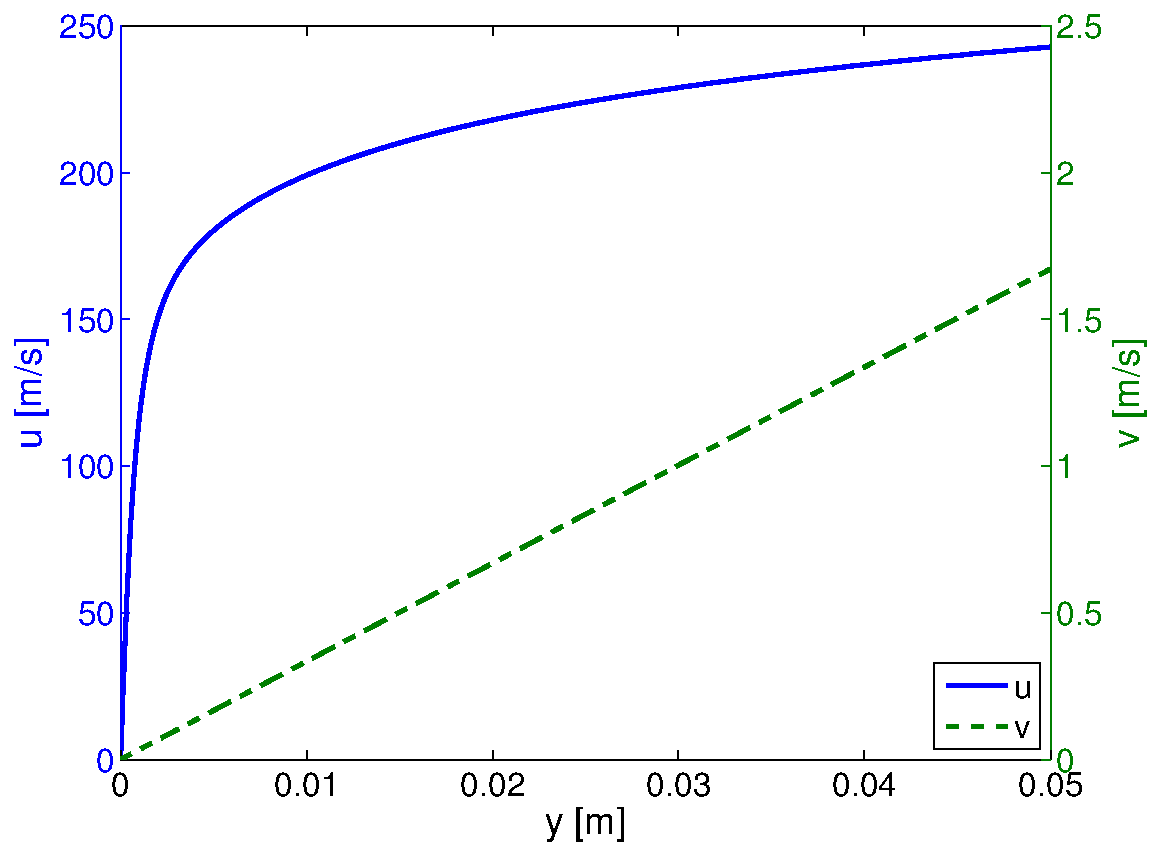
\includegraphics[width=0.5\linewidth]{figs/velocity_soln.pdf} \label{fig:velocity}}
\subfigure[The manufactured density and temperature profiles.]{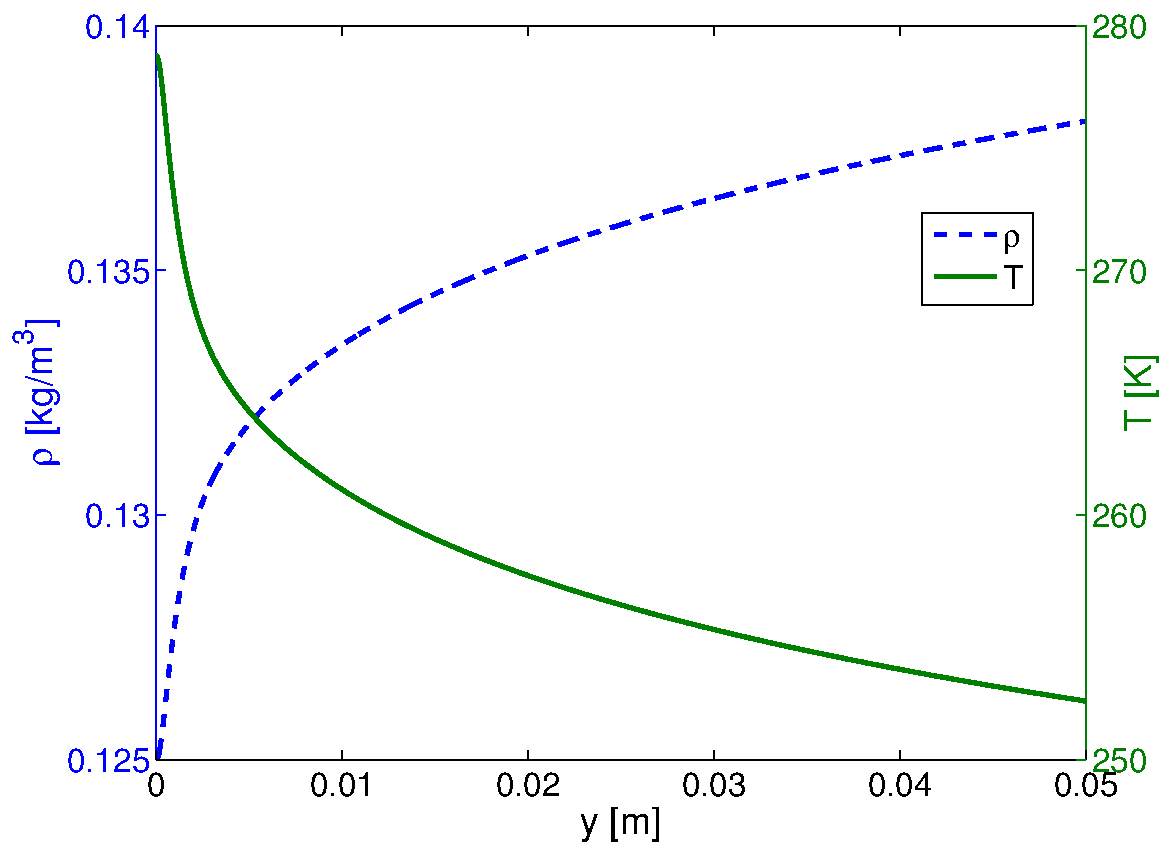
\includegraphics[width=0.5\linewidth]{figs/thermo_soln.pdf}\label{fig:thermo}}
\subfigure[The manufactured $\sa$ and $\chi$ profiles.]{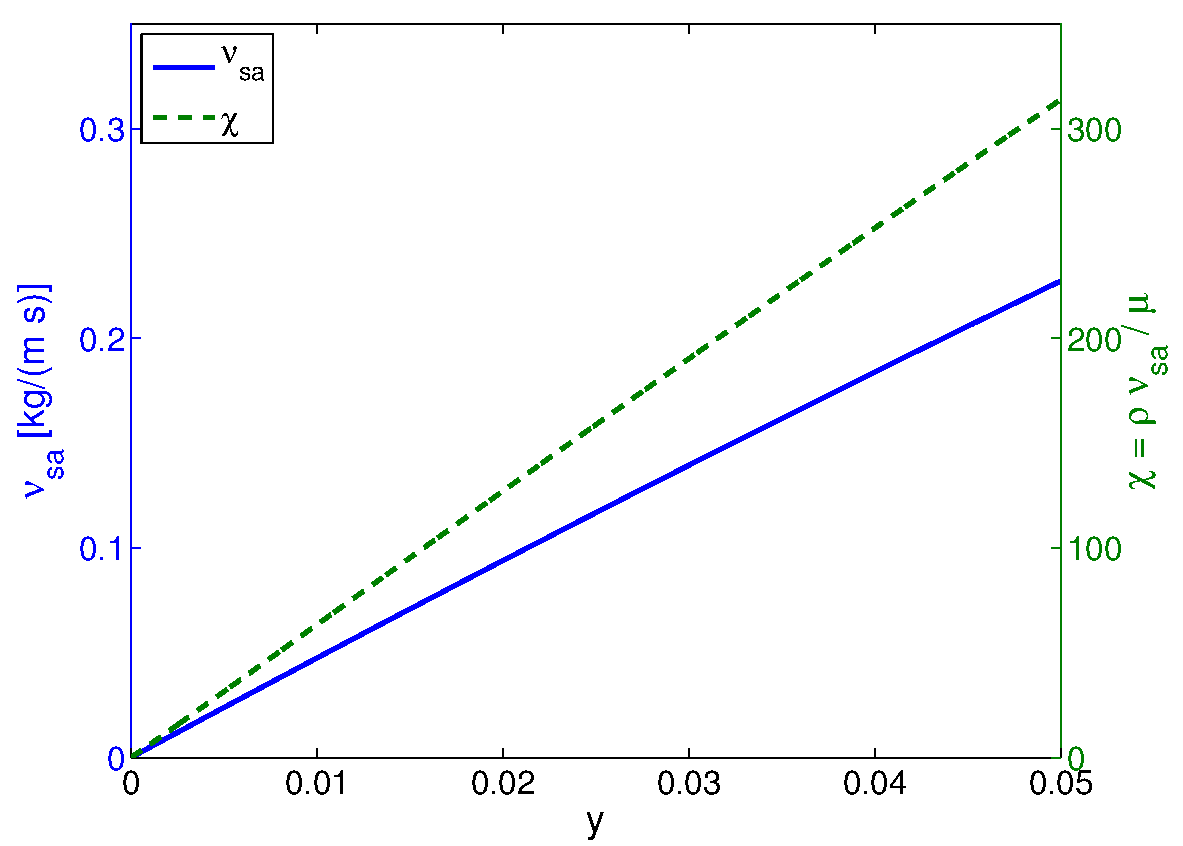
\includegraphics[width=0.5\linewidth]{figs/sa_var_soln.pdf} \label{fig:sa_profile}}
\end{center}
\vspace{-15pt}
\caption{Manufactured solutions profiles.}
\end{figure}

%
\section{SA Equation Budget} \label{sec:sa_budget}
The stated goal of this work is to develop a manufactured solution
that reasonably resembles a boundary layer.  This is most crucial with
respect to the turbulence model.  As demonstrated by \citet{Eca2007a}, the
observed behavior of the turbulence model can be highly sensitive to
the chosen manufactured solution.  To evaluate the current choices, we
plot the SA model equation budget.  The figures was generated using
the parameter values given in Section~\ref{sec:soln_plots}.  The curve
labeled ``Sum'' is equal to the sum of all of the SA terms collected
on the left hand side---i.e., it is the residual of the SA equation
evaluated at the manufactured state.  This residual is equivalent
to the source term that must be added to the right hand side to
balance the equation such that the manufactured state is a solution.
%
\begin{figure}[htp]

\begin{center}
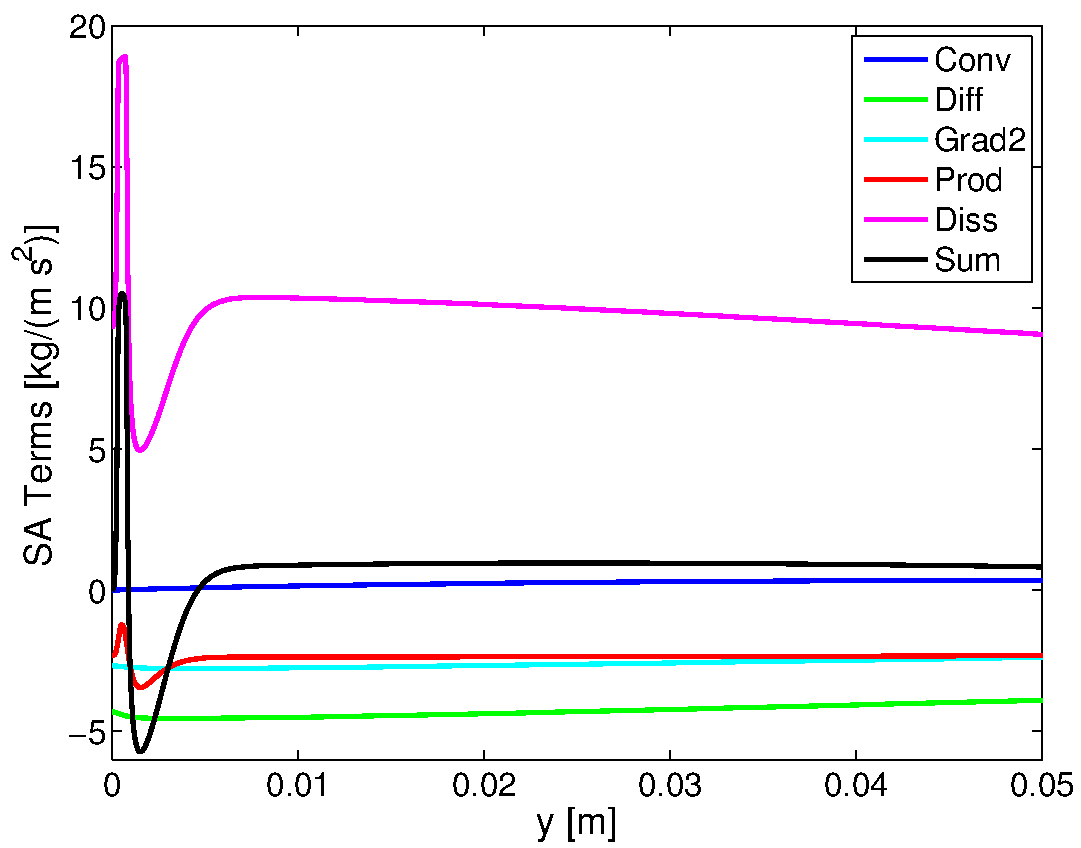
\includegraphics[width=0.5\linewidth]{figs/sa_budget.pdf}
\end{center}
\vspace{-15pt}
\caption{The Spalart-Allmaras model equation budget.}\label{fig:sa_budget}
\end{figure}

Figure \ref{fig:sa_budget} shows that for $y > 0.006 \, \mathrm{m} \approx 100
\ell_v$ the expected log layer behavior is roughly achieved.  All of
the SA terms except convection are significant and nearly in balance
(i.e., the residual term is significantly smaller than any of the
individual terms except convection).  For $y < 0.006 \,\mathrm{m}$,
the is residual is more significant, mostly due to the dissipation
term.  

Figure~\ref{fig:sa_budget_near_wall} shows the budget in this
region more clearly.
Very close to the wall ($0 \leq y \leq 1 \times 10^{-4} \approx 2
\ell_v$) the terms have the behavior expected in the viscous sublayer,
and the residual is small.  It appears that the large residual region
is associated with the transition from viscous sublayer behavior to
log layer behavior.  There is no reason to expect that the
manufactured solution constructed in this work is close to the true SA
model solution in this region.  Thus, it is reasonable for the SA
equation to be more out of balance, leading to the
larger residual in this region.
%
\begin{figure}[htp]
\begin{center}
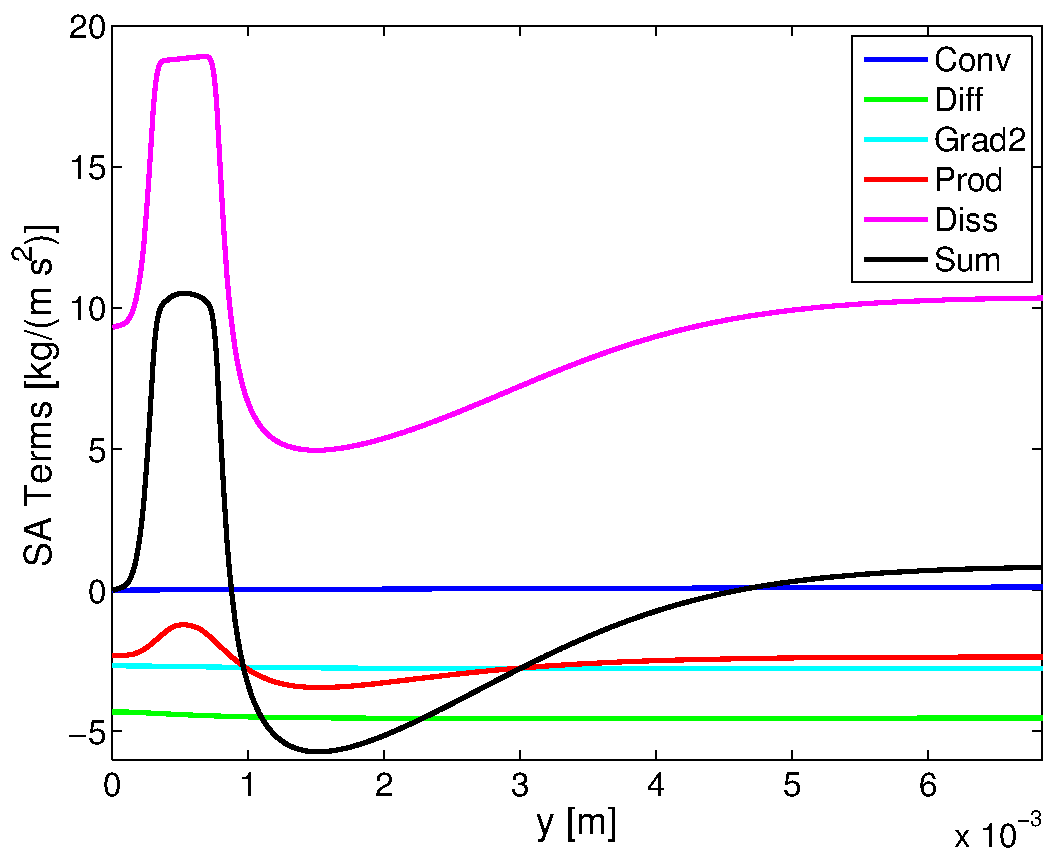
\includegraphics[width=0.5\linewidth]{figs/sa_budget_near_wall.pdf}
\end{center}
\vspace{-15pt}
\caption{The Spalart-Allmaras model equation budget very close to the wall ($0 \leq y \leq 100 \ell_v$).}\label{fig:sa_budget_near_wall}
\end{figure}
% 